\section{Nutzerdokumentation}
\subsection{Anmeldung}
Als Startseite gibt es eine Oberfläche, auf der man sich mit seiner Email-Adresse und einem Passwort anmelden muss. Das Passwort wird von einem Administrator übergeben. Dieser benötigt die Email-Adresse, um einen Account zu erstellen. Nach der Anmeldung kommt man auf die Startseite unseres Programms. Die Menüleiste besteht aus verschiedenen Knöpfen, über die der Nutzer auf Fächer, Zirkel, Schulen, Schüler oder das aktuelle Schuljahr zugreifen kann.

\begin{figure}[ht]
	\centering
	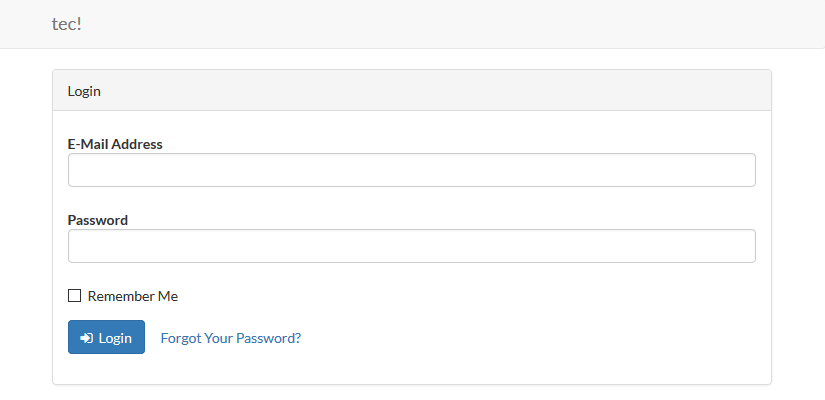
\includegraphics[scale=.48]{bilder/Anmeldung.png}
	\caption{Anmeldung}
	%\label{abb:beispiel}
\end{figure}

\subsection{Abmeldung}
Um sich abzumelden, geht man rechts oben auf seinen Nutzernamen, klickt drauf und es erscheint ein Log-out-Button.

\begin{figure}[ht]
	\centering
	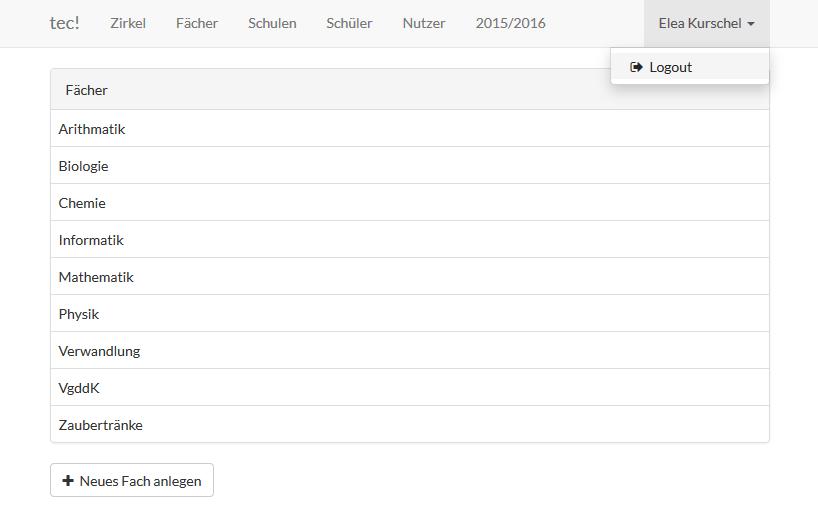
\includegraphics[scale=.48]{bilder/Abmeldung_Faecher.png}
	\caption{Abmeldung und Fächer}
	%\label{abb:beispiel}
\end{figure}

\subsection{Fächer}
Über den Fächer-Knopf kommt man auf eine Seite, auf welcher alle bisherigen angelegten Fächer aufgelistet sind. Wenn der Nutzer auf ein Fach drauf klickt, folgt eine Seite, um das Fach bearbeiten zu können. Dort kann man lediglich den Namen des Fachs ändern zum Beispiel bei einem Rechtschreibfehler. Um die Änderung zu speichern, drückt man auf den grünen Speicherbutton. Danach wird man auf die Übersichtseite der Fächer zurück geführt. Unter der Liste gibt es einen Knopf zum Anlegen neuer Fächer. Um ein neues Fach anlegen zu können, muss man nur den Namen des Fachs eintragen und auf den Anlege-Button drücken. Auch danach kommt man auf die Übersichtsseite zurück. Wenn der Nutzer ein Fach anlegt, welches schon existiert, dann kommt eine Fehlermeldung, dass der Name bereits vergeben wurde.

\subsection{Schulen}
Wenn man auf den Schulen-Knopf drückt, gelangt der Nutzer auf eine Seite mit allen Schulen, für die Schüler angemeldet wurden. Die Tabelle besteht aus dem Schulnamen und der Adresse. Auch hier kann man über eine Klick auf eine bestimmte Schule zu weiteren Daten der Schule kommen. Man gelangt zu einer Seite, wo die Schule und deren Adresse stehen und die aktiven Teilnehmer aus dieser Schule aufgelistet sind. Dort kann man über einen Löschen-Knopf die Schule löschen. Auch gibt es einen Zurück-Knopf, dieser bringt den Nutzer zur Hauptseite der Schulen zurück. Um eine neue Schule anlegen zu wollen, muss man den Neue-Schule-anlegen-Knopf betätigen. Nun muss man die geforderten Daten eingeben und schließlich auf "`Anlegen"' drücken. Ein Nutzer kann eine Schule anlegen, dabei die Adresse aber weglassen. Jedoch muss immer das Namensfeld für die Schule ausgefüllt werden, sonst kommt eine Fehlermeldung.

\begin{figure}[ht]
	\centering
	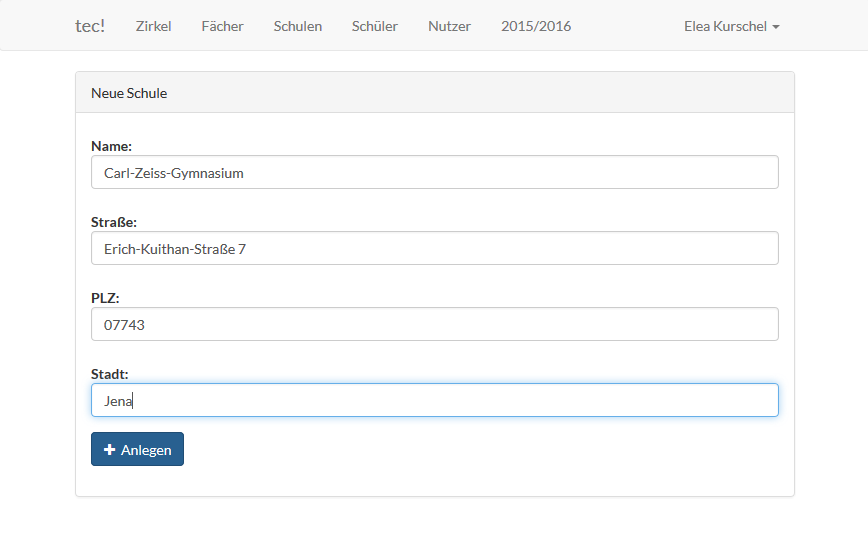
\includegraphics[scale=.45]{bilder/Neue_Schule_anlegen.png}
	\caption{Neue Schule anlegen}
	%\label{abb:beispiel}
\end{figure}

\newpage \subsection{Schüler}
Wenn der Nutzer alle Schüler aufgelistet haben möchte, muss er einfach den Schüler-Knopf auf der Menüleiste drücken. Nun sieht er alle Schüler, die eingetragen worden. Außerdem die dazugehörige Klasse, Schule und Adresse. Um die Daten eines Schülers zu bearbeiten, drückt man auf den Bereich des gewünschten Schülers. Danach sieht man noch einmal die Daten zum Schüler, einen Zurück-Knopf und kann über den Bearbeiten-Knopf den Schüler anpassen.\\
\begin{figure}[ht]
	\centering
	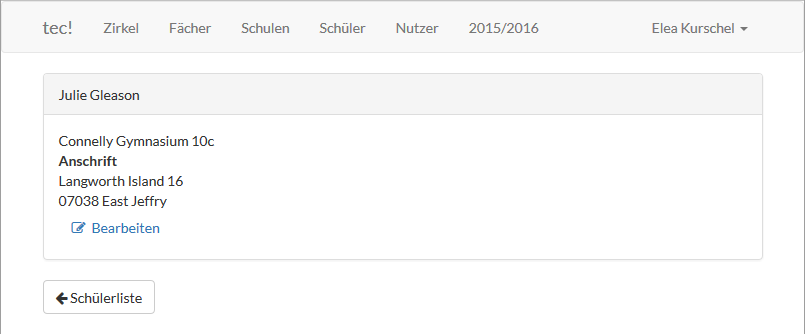
\includegraphics[scale=.5]{bilder/Schueler_Daten.png}
	\caption{Schüler mit persönlichen Daten}
	%\label{abb:beispiel}
\end{figure}
\\Um einen Schüler hinzuzufügen, klickt man auf den passenden Neuen-Schüler-hinzufügen-Knopf. Man muss immer den Vornamen, Nachnamen, die Klassenstufe und eine Schule angeben, sonst erscheint eine Fehlermeldung. Die Schule kann aus den bereits eingetragenen Schulen ausgewählt werden. Die Anschrift sowie die Klasse kann weggelassen werden. Um nicht jedes Schuljahr die Klassenstufe eines Schülers ändern zu müssen, wird über eine interne Rechnung die momentane Klassenstufe des Schülers berechnet. Dabei wird das Einschulungsjahr und das aktuell eingestellte Schuljahr verwendet.

\subsection{Zirkel}
Möchte der Nutzer alle Zirkel sehen, die dieses Schuljahr laufen, dann klickt er auf den Zirkel-Knopf in der Menüleiste. Neben dem Zirkel-Fach sieht man auch die Klassenstufe. Über den Neuen-Zirkel-Button gelangt man zu einer Seite um einen neuen Zirkel anlegen zu können. Man muss das Fach und die Klassenstufe auswählen und dann auf "`Anlegen"' drücken. Dann sieht man die Hauptseite mit den "`alten"' Zirkeln und dem neuen Zirkel. Klickt man auf einen Zirkel, wird man auf eine Seite weitergeleitet mit allen Schülern, die an diesem Zirkel teilnehmen. Unter der Tabelle befinden sich 3 Knöpfe. Links einen Knopf zum Teilnehmer verwalten und einen weitere zum Aufgaben verwalten.\\
\begin{figure}[ht]
	\centering
	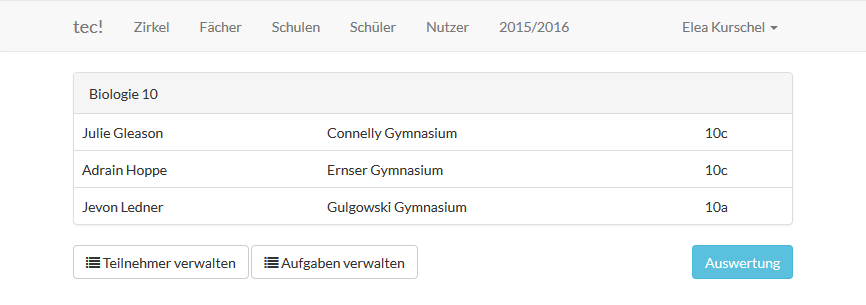
\includegraphics[scale=.5]{bilder/Zirkel_Biologie.png}
	\caption{Beispiel Biologie-Zirkel Klasse 10}
	\label{abb:beispiel}
\end{figure}
\\Über den Teilnehmer-verwalten-Knopf gelangt man zu der Seite, wo man Teilnehmer über den passenden Button ein- und austragen kann und Schüler aus einer bestimmten Klassenstufe angeben lassen kann. Man muss dazu die Klassenstufe auswählen, wobei man auch ein Stufe höher oder niedriger als die vorgesehene Klassenstufe einstellen und über das Drücken des Anzeige-Buttons anzeigen lassen kann.\\
\begin{figure}[ht]
	\centering
	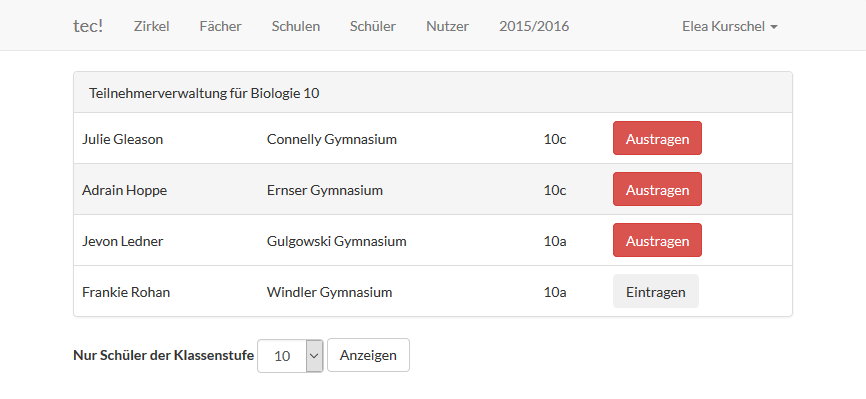
\includegraphics[scale=.5]{bilder/Teilnehmer_verwalten.png}
	\caption{Teilnehmer verwalten}
	%\label{abb:beispiel}
\end{figure}
\newpage Der Aufgaben-verwalten-Knopf bringt einen zu einer Seite, wo alle Aufgabenserien und die maximal Punktzahl dieser Serie aufgelistet sind.\\
\begin{figure}[ht]
	\centering
	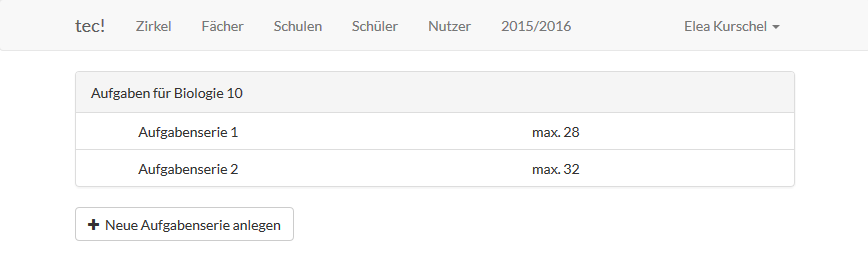
\includegraphics[scale=.5]{bilder/Aufgaben_verwalten.png}
	\caption{Aufgaben verwalten}
	%\label{abb:beispiel}
\end{figure}
\\Drückt man auf das Feld dieser Aufgabengruppe, kommt man zur Bearbeitungsseite dieser Aufgabenserie. Man kann die maximale Punktzahl verändern und für jeden Schüler, der bei diesem Zirkel mit knobelt, die erreichte Punktzahl eintragen.\\
\begin{figure}[ht]
	\centering
	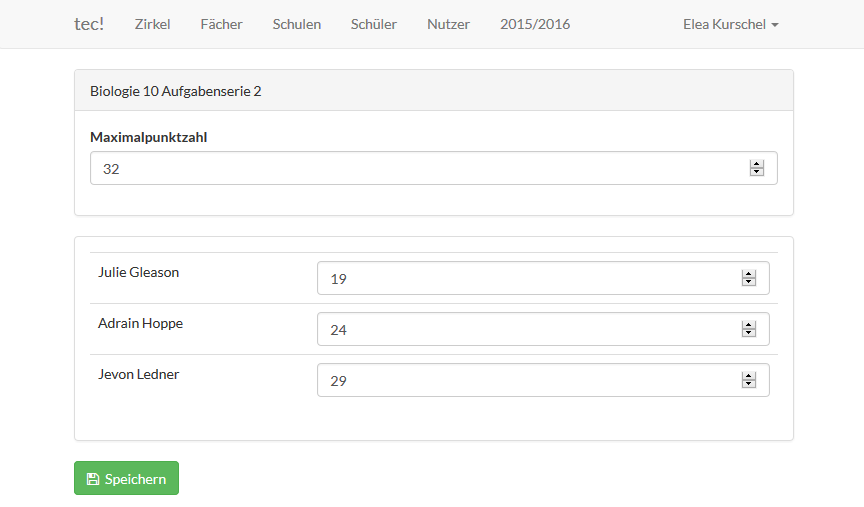
\includegraphics[scale=.5]{bilder/Aufgabenserie.png}
	\caption{Punkteverteilung}
	%\label{abb:beispiel}
\end{figure}
\\Klickt man auf "`Speichern"', wird alles gespeichert und es wird ein Liste angezeigt. Diese Liste hat alles ausgewertet, was eingetragen wurde. Es wird der Name des Teilnehmers angezeigt, für jede Aufgabeserie die erreichte Punktzahl und die Maximalpunktzahl sowie die prozentuale Erfolgsquote.\\
\begin{figure}[ht]
	\centering
	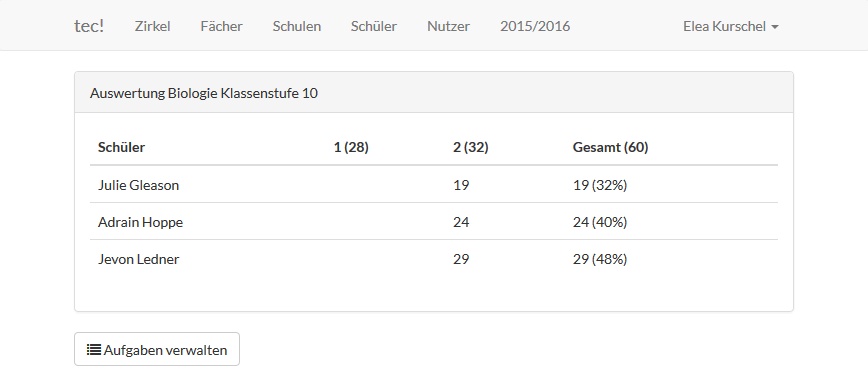
\includegraphics[scale=.5]{bilder/Auswertung.png}
	\caption{Auswertung}
	%\label{abb:beispiel}
\end{figure}
\\Über den Aufgaben-verwalten-Knopf gelangt man wieder zurück zur vorherigen Seite. Wenn man auf der Seite für ein bestimmten Zirkel ist und den Auswertung-Button drückt, kommt man auch auf die Seite für die Auswertung. Wenn hier auf einen Teilnehmer gedrückt wird, dann kommt man auf die Daten des Schülers (siehe Schüler).

\begin{figure}[ht]
	\centering
	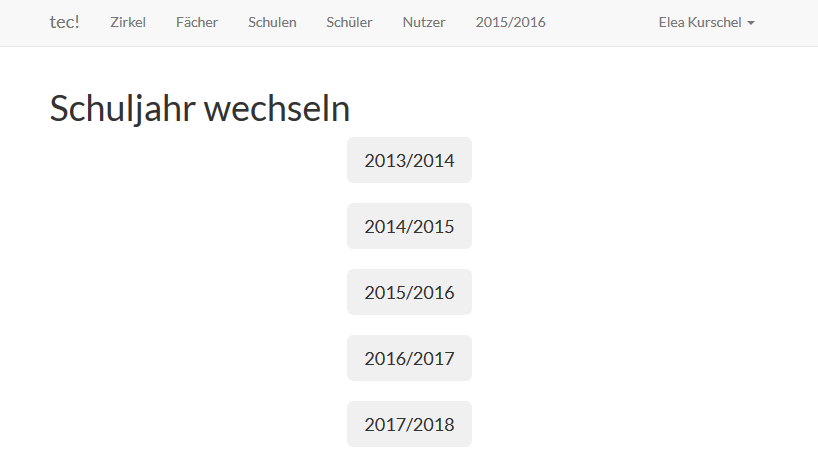
\includegraphics[scale=.40]{bilder/Schuljahr.png}
	\caption{Schuljahr wechseln}
	%\label{abb:beispiel}
\end{figure}

\subsection{Schuljahr}
Oben in der Menüleiste wird auch das aktuelle Schuljahr angezeigt. Um das Schuljahr zu wechseln, klickt man einfach auf den Knopf und kommt zur passenden Seite. Nun werden das aktuelle aber auch die 2 Schuljahre davor und die 2 zukünftigen angezeigt. Jetzt wählt man sein gewünschtes Schuljahr aus, alle Daten werden angepasst und man findet sich auf der Startseite wieder.


\subsection{Nutzer}
Ein Admin kann zusätzlich über einen Nutzer-Button auf die Nutzer zugreifen und diese verwalten. Die Nutzer sind mit ihrem Namen, der Email-Adresse und ob sie Admin sind aufgelistet. Wenn man einen neuen Account für jemanden hinzufügen will, dann klickt man auf "`Neuen Nutzer anlegen"'. Nun muss man den Namen, die Email-Adresse und das Passwort eingeben. Außerdem kann man noch über ein Kästchen festlegen, ob der neue Nutzer ein Administrator ist oder nicht. Wenn man den Namen, die Email-Adresse oder das Passwort weglässt, erscheint eine Fehlermeldung. Das Passwort muss mindestens 6 Zeichen lang sein. Wenn man nun erfolgreich einen neuen Nutzer angelegt hat und auf speichern drückt, sieht man erneut die Liste aller Nutzer. Um die Daten eines Nutzers zu ändern, muss einfach auf das Feld des Nutzers geklickt werden. Es wird eine neue Seite aufgerufen. Man kann hier einen schon vorhandenen Nutzer zum Admin machen oder den Nutzer über den roten Löschen-Knopf löschen. Nachdem man auf "`Speichern"' oder "`Löschen"' drückt, wird wieder die Nutzerliste angezeigt. 

\begin{figure}[ht]
	\centering
	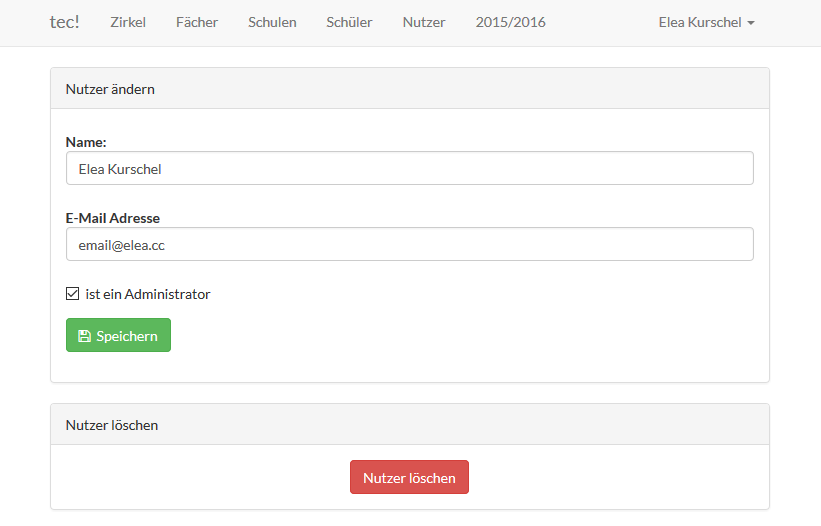
\includegraphics[scale=.5]{bilder/Nutzer.png}
	\caption{Nutzer}
	%\label{abb:beispiel}
\end{figure}